\chapter{Statistical Interpretations of the Data}
\label{chap:statistics}

When searching for new physics it is often desirable to do so in the context of
some specific theoretical model or well motivated benchmark scenario.
Where the theory provides well defined predictions,
experimental data can be used to verify or reject the theory
by means of hypothesis testing. This chapter describes the frequentist statistical procedures 
employed at CMS to perform these tests and provide quantitative, statistical interpretations  
of the data. In Section~\ref{sec:hypothesistesting}, an overview is given on the procedure by 
which $p$-values are calculated to test the compatibility of the data with a given 
hypothesis and the $CL_{s}$ technique for setting exclusion limits is introduced. 
The results of applying these procedures to the $\Hgg$ analysis described in Chapter~\ref{chap:hgg} 
are given in Section~\ref{sec:hggresults2011} including updates for the 8 TeV using data taken 
in 2012 up to the ICHEP conference that year.


\section{Hypothesis Testing}
\label{sec:hypothesistesting}

The goal is to use the data 
to reject one of two hypotheses,
$H_{0}$ and $H_{1}$, known as the null and alternate hypotheses
respectively. A function is defined, $t(data)$,
which characterises the observed data as a single real value. When rejecting 
the hypothesis, $H_{0}$, the critical
region, $w$, is defined as the set of possible values of $t$
which indicate that $H_{0}$ is not true. The probability then 
to observe $t\in w$ when $H_{0}$ is true ($\alpha$), 
\begin{equation}
\alpha = P(t\in w|H_{0})
\end{equation}
is the probability that $H_{0}$ would be rejected even if it was true.
The strength of a test (referred to as its power) is quantified by 
the probability, $1-\beta$ that $t \in  w$ when $H_{1}$ is true.
\begin{equation}
1-\beta = P(t\in w|H_{1})
\end{equation}
In the case of the search of the SM Higgs boson, the two hypotheses
can be parameterised in terms of a production cross-section relative
to that predicted by the SM, $\xs$.  
The null hypothesis ($H_{0}$) is then that under which no SM Higgs boson exits,
$\xs=0$, while the alternate ($H_{1}$) is characterized by $\xs=1$.
In this case, $H_{0}$ is referred to as the background-only hypothesis
and $H_{1}$ the signal-plus-background hypothesis.
The possible outcomes of $t$ are assumed to be random with a probability density
function (pdf) $f_{\xs}(t)$. The values of $\alpha$ and $1-\beta$ are the integral of the pdfs
over the critical region;
\begin{eqnarray}
1-\beta =  \int_{w}f_{1}(t)dt\\ 
\alpha =  \int_{w}f_{0}(t)dt.
\label{eqn:alpha}
\end{eqnarray}
It can be shown that the choice of $w$ which maximises the power of the test for 
a given value of $\alpha$ are the set of points for which,
\begin{equation} 
	q = \frac {\displaystyle f_{1}(t)}{\displaystyle f_{0}(t)} \ge c_{\alpha},
\label{eqn:bestw}
\end{equation}
where $c_{\alpha}$ is chosen such that Equation~\ref{eqn:alpha} holds~\citep{statsbook}.
In the search for the SM Higgs boson, the compatibility of the data
with the presence of a Higgs boson is interpreted in terms of the 
continuous parameter, $\mu$, which scales the signal strength relative to that expected
from the Standard Model. 
Again, the null hypothesis, $H_{0}$, is characterized by setting $\mu=0$ however,
an infinite number of alternate hypotheses exist for any value $\mu \ge 0$.
The likelihood , $\call(t|\mu)$, is defined as a function of $\mu$ for a fixed 
realisation of the data and related to each pdf by a constant of proportionality.
The quantity $q$ in Equation~\ref{eqn:bestw}, known as the ``test-statistic'', is then
the ratio of the likelihood at the two values $\mu=1$ and $\mu=0$. 

The test-statistic for a given $\mu$ is defined as the ratio 
of likelihoods, $q_{\mu}$, in which the values for the nuisance parameters are taken from fits to the data (profiled), 
as given in Equation~\ref{eqn:llr2}. 
\begin{equation}
\qmu = 
	\begin {cases} 
	-2\ln\frac{\displaystyle \mathcal{L}(\mathrm{data} | \mu,\hat{\boldth}_{\mu})}
	{\displaystyle \mathcal{L}(\mathrm{data} | \muhat,\hat{\boldth})} 
		&  0 \le \muhat \le \mu \\
	 0 	&  \muhat < 0
	\end{cases}.
\label{eqn:llr2}
\end{equation}
The values $\hat{\boldth}_{\mu}$ and $\hat{\boldth}$ are the values of 
the nuisance parameters for which the likelihood attains its maximum 
given a particular value of $\mu$ and letting $\mu$ to float freely in the 
fit ($\mu=\muhat$).
An immediate consequence of this definition is that the value attained
by the test statistic is always positive. Small values of the test
statistic indicate outcomes which are in favour of the signal-plus-background 
hypothesis, where large values indicate outcomes which disfavour it.
Due to this, the critical region $w$ can always be defined as the right
hand tail of the normalized distribution of the test-statistic $f(q_{\mu}|\mu)$, 
\begin{equation}
w = \left\{ q_{\mu} : q_{mu} \in (c_{\alpha},+\infty) \right\},
%\label{eqn:llr2}
\end{equation}
Commonly the integral of $f(q_{\mu}|\mu)$ above the observed value of the 
test-statistic in data $(q_{\mu}^{obs})$, known as a $p$-value, is calculated
to provide a measure of how much the data disfavour a particular value of $\mu$. 

\subsection{Exclusion Limits}
An upper limit ($\mu_{up}$) can be determined for $\mu$ such that
the hypotheses represented by the set $\left\{ \mu:\mu>\mu_{up} \right\}$
are nested (contained) within the hypothesis represented by $\xs=\mu=>\mu_{up}$.
For the special case when $\mu_{up}=1$, the presence of a SM Higgs boson is excluded
(at some confidence level $c\in(0,1)$) in favour of the background-only hypothesis. 
The constraint of $\muhat \le \mu$ is imposed in the chosen test-statistic, $q_{\mu}$,  
when calculating upper limits which forces the limit on $\mu$ to be one-sided.
At CMS, upper limits are determined using the $CL_{s}$
which is designed to provide less stringent exclusion limits in analyses 
which are less sensitive to signal~\citep{cls}. 
This procedure involves computing two $p$-values (tail probabilities) under two hypothesis, $\mu=0$ and $\mu\ne0$ given by,
\begin{equation}
	CL_{s+b} = \int_{\qmu^{obs}}^{\infty} f(\qmu | \mu,\boldth=\boldth_{\mu}^{obs}) d\qmu
\label{eqn:clsplusb}
\end{equation}
\begin{equation}
	CL_{b} = \int_{\qmu^{obs}}^{\infty} f(\qmu |0,\boldth=\boldth_{0}^{obs}) d\qmu,
\label{eqn:clb}
\end{equation}
where $q_{\mu}^{obs}$ is the value of the test-statistic in data. 
The smallest value of $\mu$ for which the ratio $CL_{s}=\frac{\displaystyle CL_{s+b}}{\displaystyle CL_{b}}<\alpha$ is quoted as the upper limit on $\mu$ with confidence level 
$1-\alpha$. Typically, for exclusion, $\alpha$ is chosen as 0.05 so that 
when the upper limit on $\mu$ is less than one, all hypotheses of $\xs\ge1$ are excluded 
at the 95\% confidence level or more. In the search for a SM Higgs boson, this corresponds to excluding 
a SM Higgs boson with a particular mass $\mh$ hypothesis under which the likelihood is constructed.
 
The distributions of the test-statistic, $\qmu$ under the two hypotheses are generated by 
throwing pseudo-experiments using the signal and background models such as those 
derived in Section~\ref{sec:signalextraction}.
First, the values of $\boldth^{obs}_{\mu}$ and $\boldth^{obs}_{0}$ are set by fitting the likelihood 
to the observed data at a particular value of $\mu$ and for $\mu=0$ respectively. Pseudo-data, $d_{j}$, for each bin
are generated according to a Poisson distribution with expectation value 
$\mu s_{j}(\boldth_{\mu}^{obs})+b_{j}(\boldth_{\mu}^{obs})$. Pseudo-measurements for each nuisance parameter,
$\boldthmeas$, are then regenerated before evaluating the
test-statistic $q_{\mu}$ in order to model the effect of systematic uncertainties. 
Examples of the normalised distributions of $\qmu$ for $\mu=0.6$ and $\mu=0$ are shown in 
Figure~\ref{fig:qmuexample}.

\begin{figure}
\begin{center}
  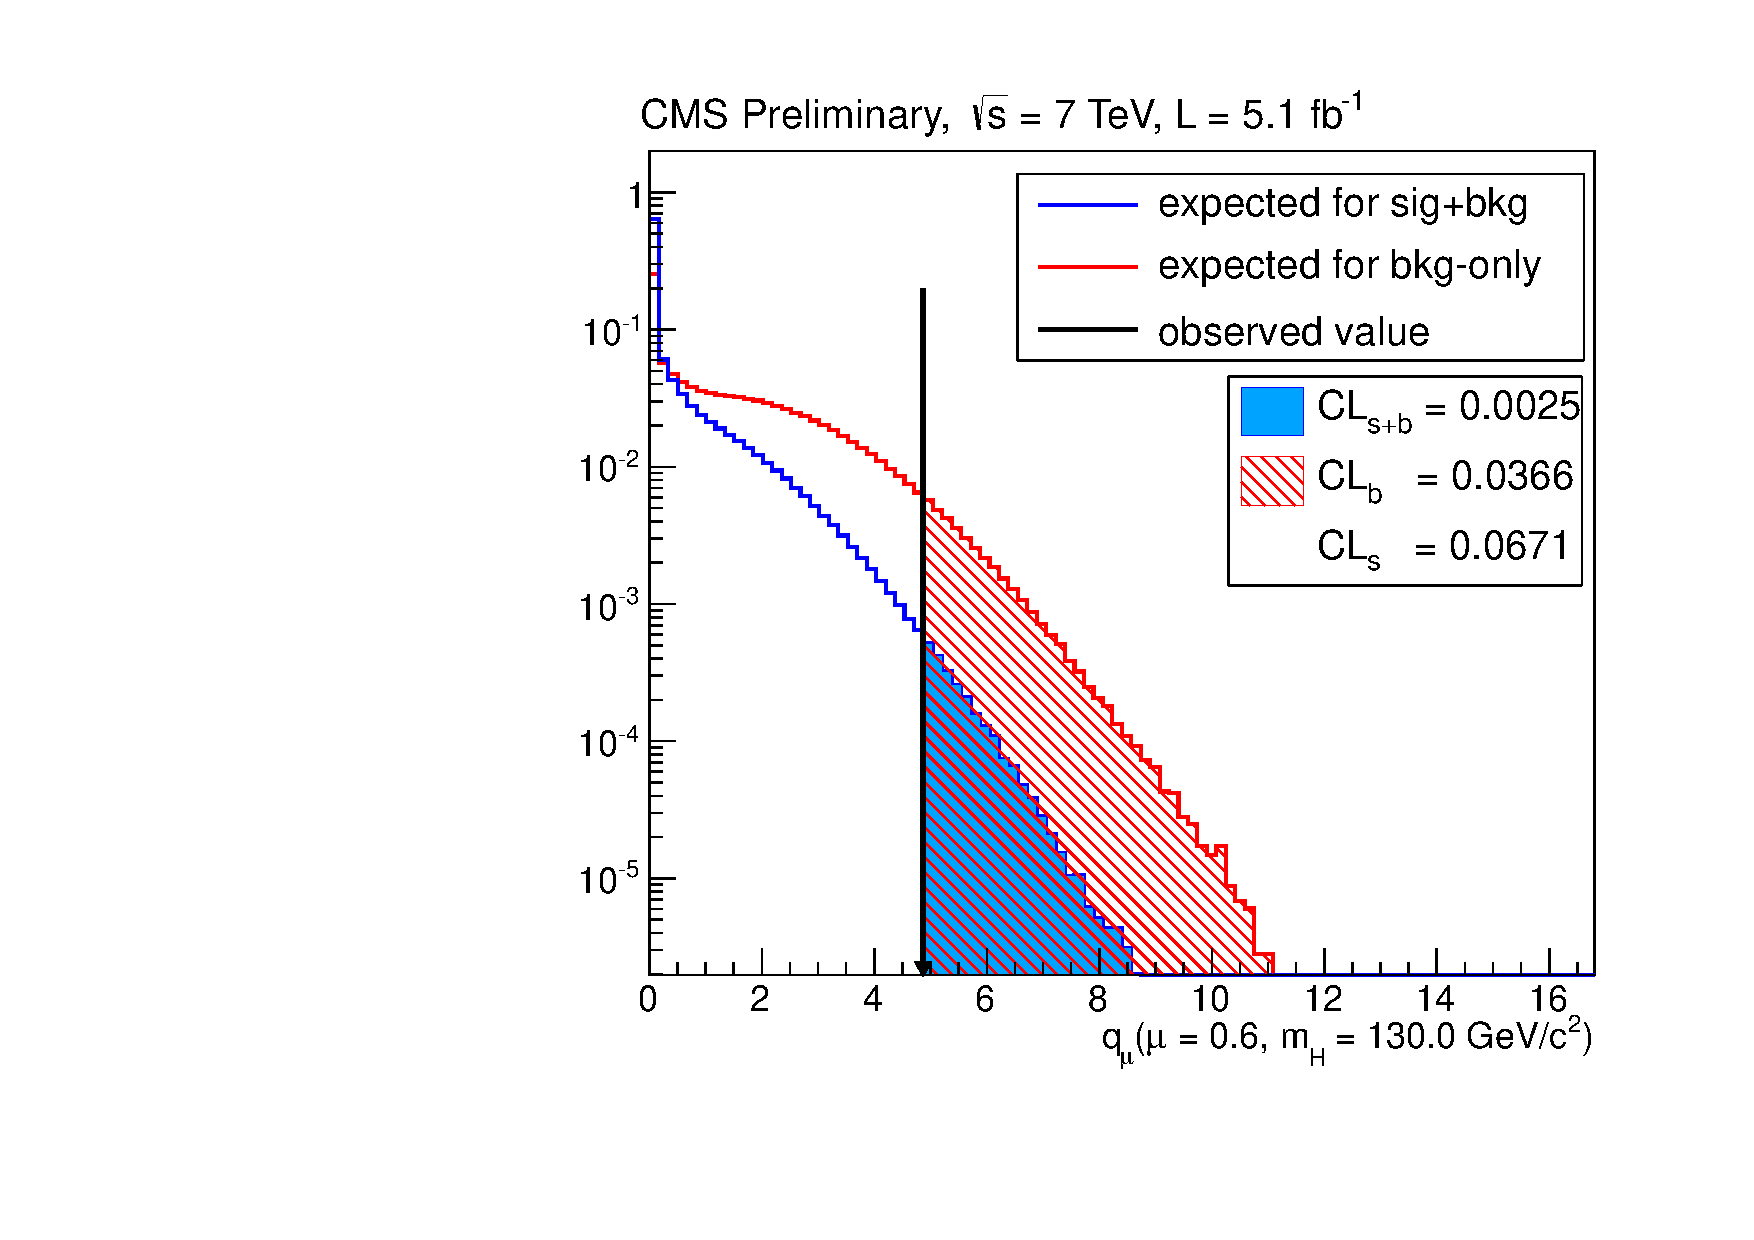
\includegraphics[width=.8\textwidth]{hgg7TeV/statsPlots/qmu_example_130.pdf}
\end{center}
 \caption{Distributions of the test statistic $\qmu$ under a background-only hypothesis
 ($\mu=0$) and signal plus background hypothesis ($\mu=0.6$) for a SM Higgs boson of mass 130 GeV. 
 The distributions are normalised to unit area. The observed value of the test statistic 
 from data is indicated by the black arrow.}
 \label{fig:qmuexample}
\end{figure}

\subsection{Quantifying Excesses in the Observed Data}

In the presence of a sizeable excess in data, the background-only hypothesis
can be rejected in favour of an signal-plus-background like one. Specifically, in 
the search for the SM Higgs boson, the excess 
will be compatible with the presence of a SM Higgs boson up to the rate
at which it is produced. This is due to the inclusion of the signal model 
in the definition of the likelihood which typically includes the shape of 
the expected signal in some discriminating variable and the relative populations
expected in different channels.
In order to quantify the excess, the test-statistic
is replaced with $q_{0}$ by setting $\mu=0$ in Equation~\ref{eqn:llr2}.
The constraint $\muhat>0$ ensures that only excesses in the data are considered significant.
The background-only hypothesis is rejected in favour of a signal-plus-background one
when the $p$-value $p_{0}$, given in Equation~\ref{eqn:plocal},
is less than some pre-determined critical level $\alpha$.
\begin{equation}
  p_{0} = \int_{q_{0}^{obs}}^{\infty} f(q_{0} |0,\boldth=\boldth_{0}^{obs}) dq_{0}.
\label{eqn:plocal}
\end{equation}
Since $p_{0}$ is uniformly distributed between 0 and 1 under the hypothesis $\mu=0$,
$p_{0}$ is exactly the probability $\alpha$ of falsely rejecting the background-only hypothesis. 
The critical value for $\alpha$ is typically $2.87\times10^{-7}$ (corresponding 
to a significance of $5\sigma$) when searching for new physics.  

In the case of the search for the SM Higgs boson, there is an implicit assumption that
the test statistic is defined for a given value of $\mh$. The test statistic designed this way
means that only excesses which are compatible in shape with that of a Higgs signal at some $\mh$
are considered significant. The $\Hgg$ signal is a narrow peak in the diphoton invariant mass distribution
meaning only localised excesses in $\mgg$ are considered significant.
The value of $p_{0}$ is therefore interpreted as the probability that the background can 
fluctuate to produce a localised excess hence $p_{0}$ is termed the local p-value.

Analogous to calculating limits, the distribution $f(q_{0} |0,\boldth=\boldth_{0}^{obs})$ can be obtained either
through generating toys or using an analytic form. Figure~\ref{fig:q0dist} shows the normalised distribution
of $q_{0}$ under the background-only hypothesis generated from pseudo-experiments compared with the 
analytic form, in this case a $\chi^{2}$ distribution with a single degree of freedom, at $m_{H}=124$ GeV.

\begin{figure}
\begin{center}
  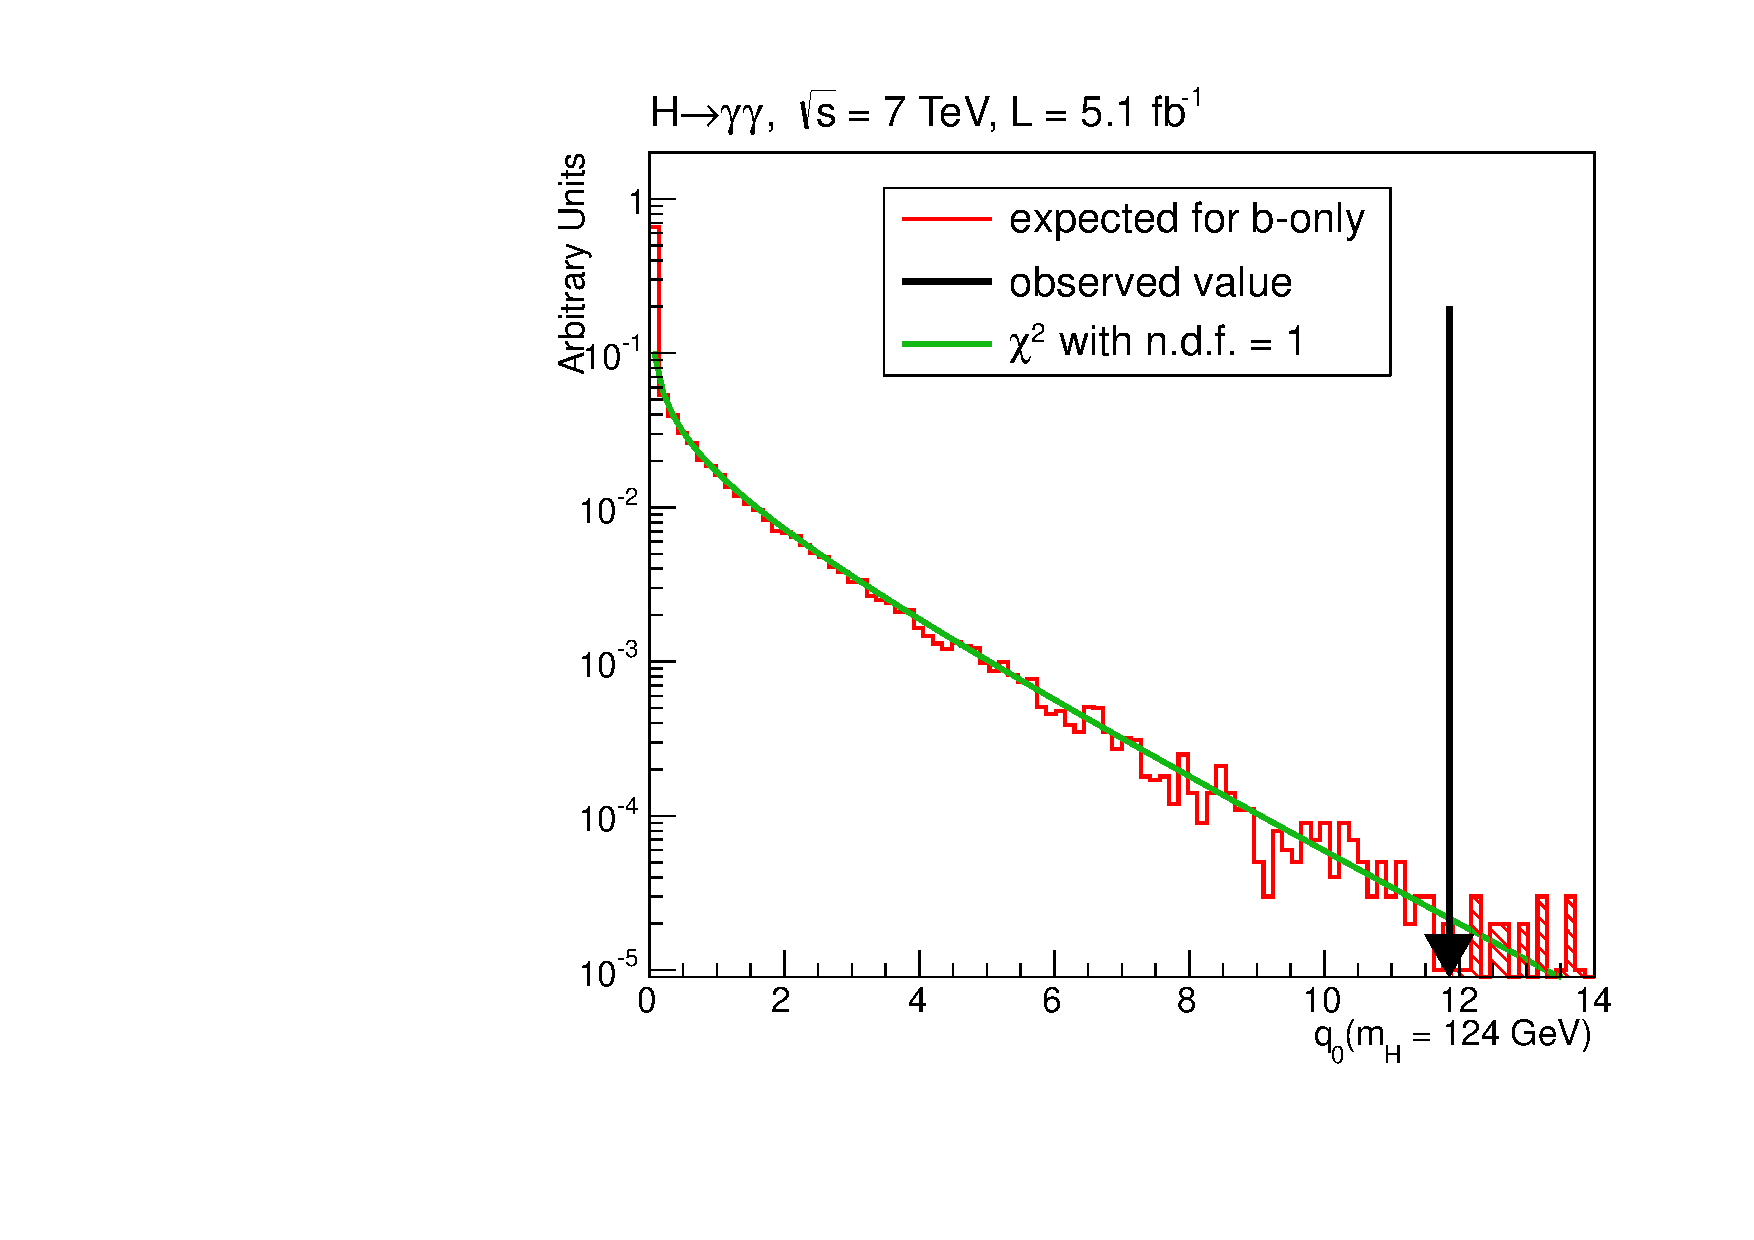
\includegraphics[width=.8\textwidth]{hgg7TeV/statsPlots/q0_example_125_chi2_sqr.pdf}
\end{center}
 \caption{Normalised distribution of $q_{0}$ at $\mh=124$ GeV under the background-only 
 hypothesis generated  from toys (red histogram) and from the analytic form (green line). 
 The observed value, $q_{0}^{obs}$, obtained from the data is indicated by the black arrow.}
 \label{fig:q0dist}
\end{figure}
 


\section{$\Hgg$ Statistical Results}
\label{sec:hggresults2011}

The likelihood in Equation~\ref{eqn:likelihoodhggbdt} was coded using the \texttt{C++} based 
statistical package \texttt{RooFit/RooStats} version \texttt{5.3.0}~\citep{roofit}. 
A framework for automating the procedure of combining datasets, generating toys
and evaluating likelihoods in the context of the combined search for the SM Higgs boson
was developed within \texttt{CMSSW} 
under the package \\
\texttt{HiggsAnalysis/CombinedLimit}~\citep{combinationstwiki}.
All of the results shown in the following sections were obtained using this package.

The 95\% confidence upper limits on $\xsbr$ were determined using the full 2011 dataset 
for different values of $\mh$ in the range to which the channel $\Hgg$ is most sensitive.
Since the resolution of the signal peak in the $\Hgg$ channel is of the order 1 GeV, the limit is calculated
in 100 MeV steps in the range $110 < \mh < 150$ GeV. Figure~\ref{fig:limits7TeV} shows the expected and observed
upper limit on the ratio $\xsbr$ in that range. Where the observed line falls below the red line
at one, a SM Higgs boson decaying to two photons, with mass $\mh$, is excluded at the 95\% confidence level or more. 
The limits were calculated using an asymptotic approximation for the distribution of $q_{\mu}$ thereby 
removing the need for generation of pseudo-experiments~\citep{asimov}. The procedure involving the generation of toys
was however conducted for several mass hypotheses and found to agree
with the asymptotic calculation. Table~\ref{tab:compareasvstoys} shows this comparison 
for the median expected, 68\% and 95\% quantile ranges at different values of $\mh$.

\begin{table}
\begin{tabular*}{0.75\textwidth}{@{\extracolsep{\fill}}|l|c|c|}\hline
 & \textbf{Toys} & \textbf{Asymptotic} \\ \hline
%  \multicolumn{3}{|l|}{$m_{H}=110$} \\ \hline
%2.5\%   & 0.64179  & 0.641275 \\ 
%16\%    & 0.398908 & 0.396169 \\ 
%median  & 1.3897   & 1.38408 \\ 
%84\%    & 0.610173 & 0.620358 \\ 
%97.5\%  & 1.41708  & 1.46024 \\ \hline 
  \multicolumn{3}{|l|}{$m_{H}=120$ GeV} \\ \hline
2.5\%  &  $0.534\pm0.044$ & 0.533 \\ 
16\%  &   $0.777\pm0.012$ & 0.778 \\ 
median &  $1.175\pm0.020$ & 1.174 \\ 
84\%  &   $1.785\pm0.021$ & 1.795 \\ 
97.5\%  & $2.592\pm0.213$ & 2.635 \\ \hline 
  \multicolumn{3}{|l|}{$m_{H}=130$ GeV} \\ \hline
2.5\%  &  $0.629\pm0.051$ & 0.605 \\ 
16\%  &   $0.822\pm0.012$ & 0.798 \\ 
median &  $1.149\pm0.019$ & 1.145 \\ 
84\%  &   $1.665\pm0.019$ & 1.663 \\ 
97.5\%  & $2.349\pm0.192$ & 2.372 \\ \hline 
  \multicolumn{3}{|l|}{$m_{H}=140$ GeV} \\ \hline
2.5\%  &  $0.855\pm0.070$ & 0.817 \\ 
16\%  &   $1.040\pm0.015$ & 1.001 \\ 
median &  $1.361\pm0.022$ & 1.346 \\ 
84\%  &   $1.869\pm0.021$ & 1.849 \\ 
97.5\%  & $2.540\pm0.208$ & 2.546 \\ \hline 
%  \multicolumn{3}{|l|}{$m_{H}=150$} \\ \hline
%2.5\%   & 0.931103 & 0.873169 \\ 
%16\%    & 0.579237 & 0.525472 \\ 
%median  & 1.86911  & 1.82842 \\ 
%84\%    & 0.837197 & 0.841986 \\ 
%97.5\%  & 1.94052  & 1.99635 \\ \hline
\end{tabular*}
\caption{Comparison of expected median upper limit and quantiles obtained using the asymptotic calculation 
of $CL_{s}$ and toys. The error quoted in the toys column is the statistical uncertainty 
from only generating 1000 toys at each value of $\mu$. 
The comparison is made at three mass hypotheses in the range 120 to 140 GeV.}
\label{tab:compareasvstoys}
\end{table}

\begin{figure}
\begin{center}
  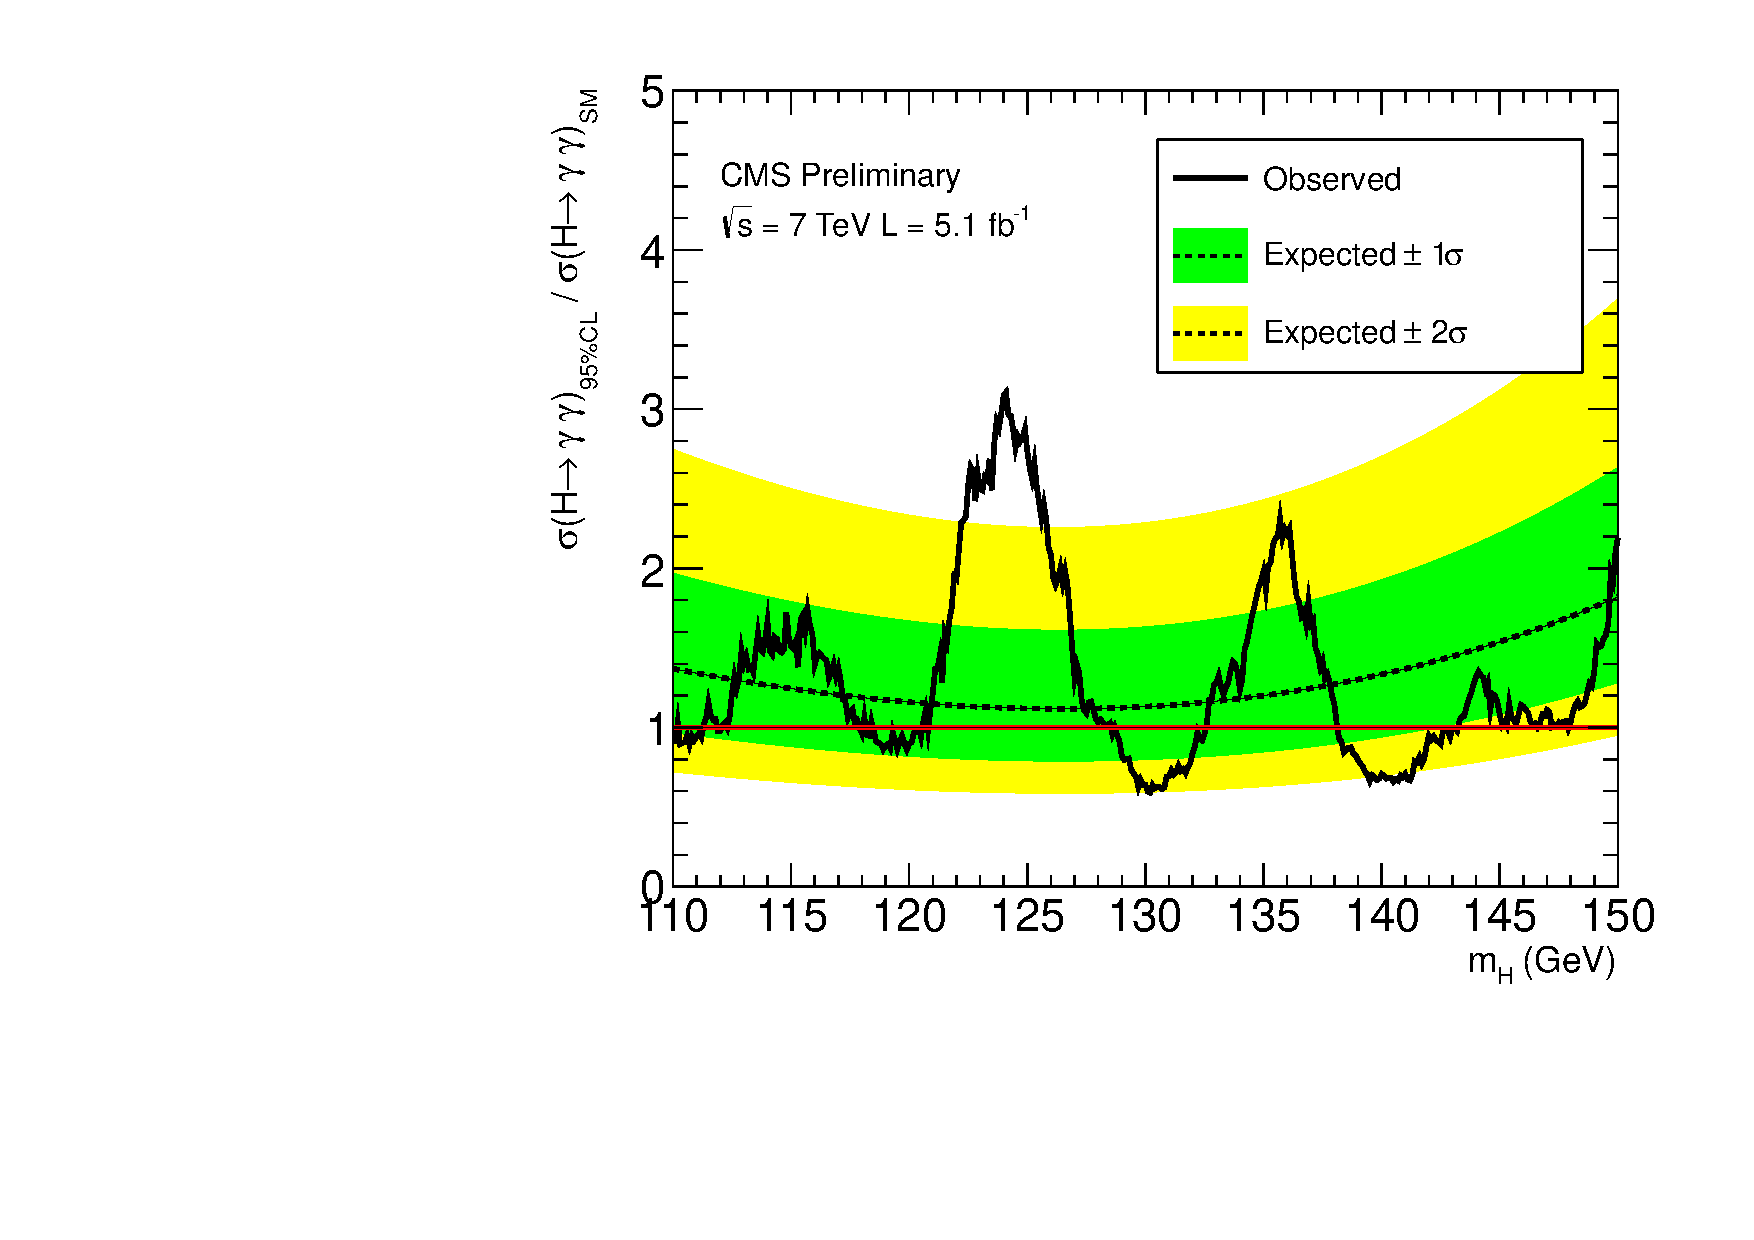
\includegraphics[width=.8\textwidth]{hgg7TeV/statsPlots/limit-100MeV.pdf}
\end{center}
 \caption{Exclusion limits on SM Higgs boson production and subsequent decay to two photons in the range
 $110 < \mh < 150$ GeV. The black dashed line indicates the median expected value for the upper limit on $\mu$
 given the size of the dataset while the green and yellow bands indicate the 68\% and 95\% quantile ranges 
 respectively.
 The black solid line shows the observed upper limit extracted from the data at steps in $\mh$ of 100 MeV. 
 Where this line falls below the red line at 1, a SM Higgs boson at that mass is excluded at the 95\% confidence level or more.}
\label{fig:limits7TeV}
\end{figure}

The local p-value from the data is determined in steps of 100 MeV in the range $100 < \mh < 150 $ GeV
using the analytic expression $p_{0} = \sqrt{q_{0}^{obs}}$
as shown in Figure~\ref{fig:pvals7TeV}. The expectation in the presence of a SM Higgs boson at each $\mh$ tested
is shown in blue while the expectation from a SM Higgs boson with mass 125 GeV is shown in red. 
The largest excess in the range occurs near $\mh=124$ GeV corresponding
to a local significance of $3.4\sigma$. The excess is larger than expected in the presence of a SM 
Higgs boson near that mass. This is reflected in Figure~\ref{fig:muhat7TeV} which shows the value of 
$\mu$ at which the likelihood attains its maximum, $\muhat$, as a function of $\mh$. 
The excess observed at 124 GeV corresponds to $\muhat=1.93^{+0.67}_{-0.60}$, that is nearly twice 
the expectation from a SM Higgs boson.

\begin{figure}
\begin{center}
  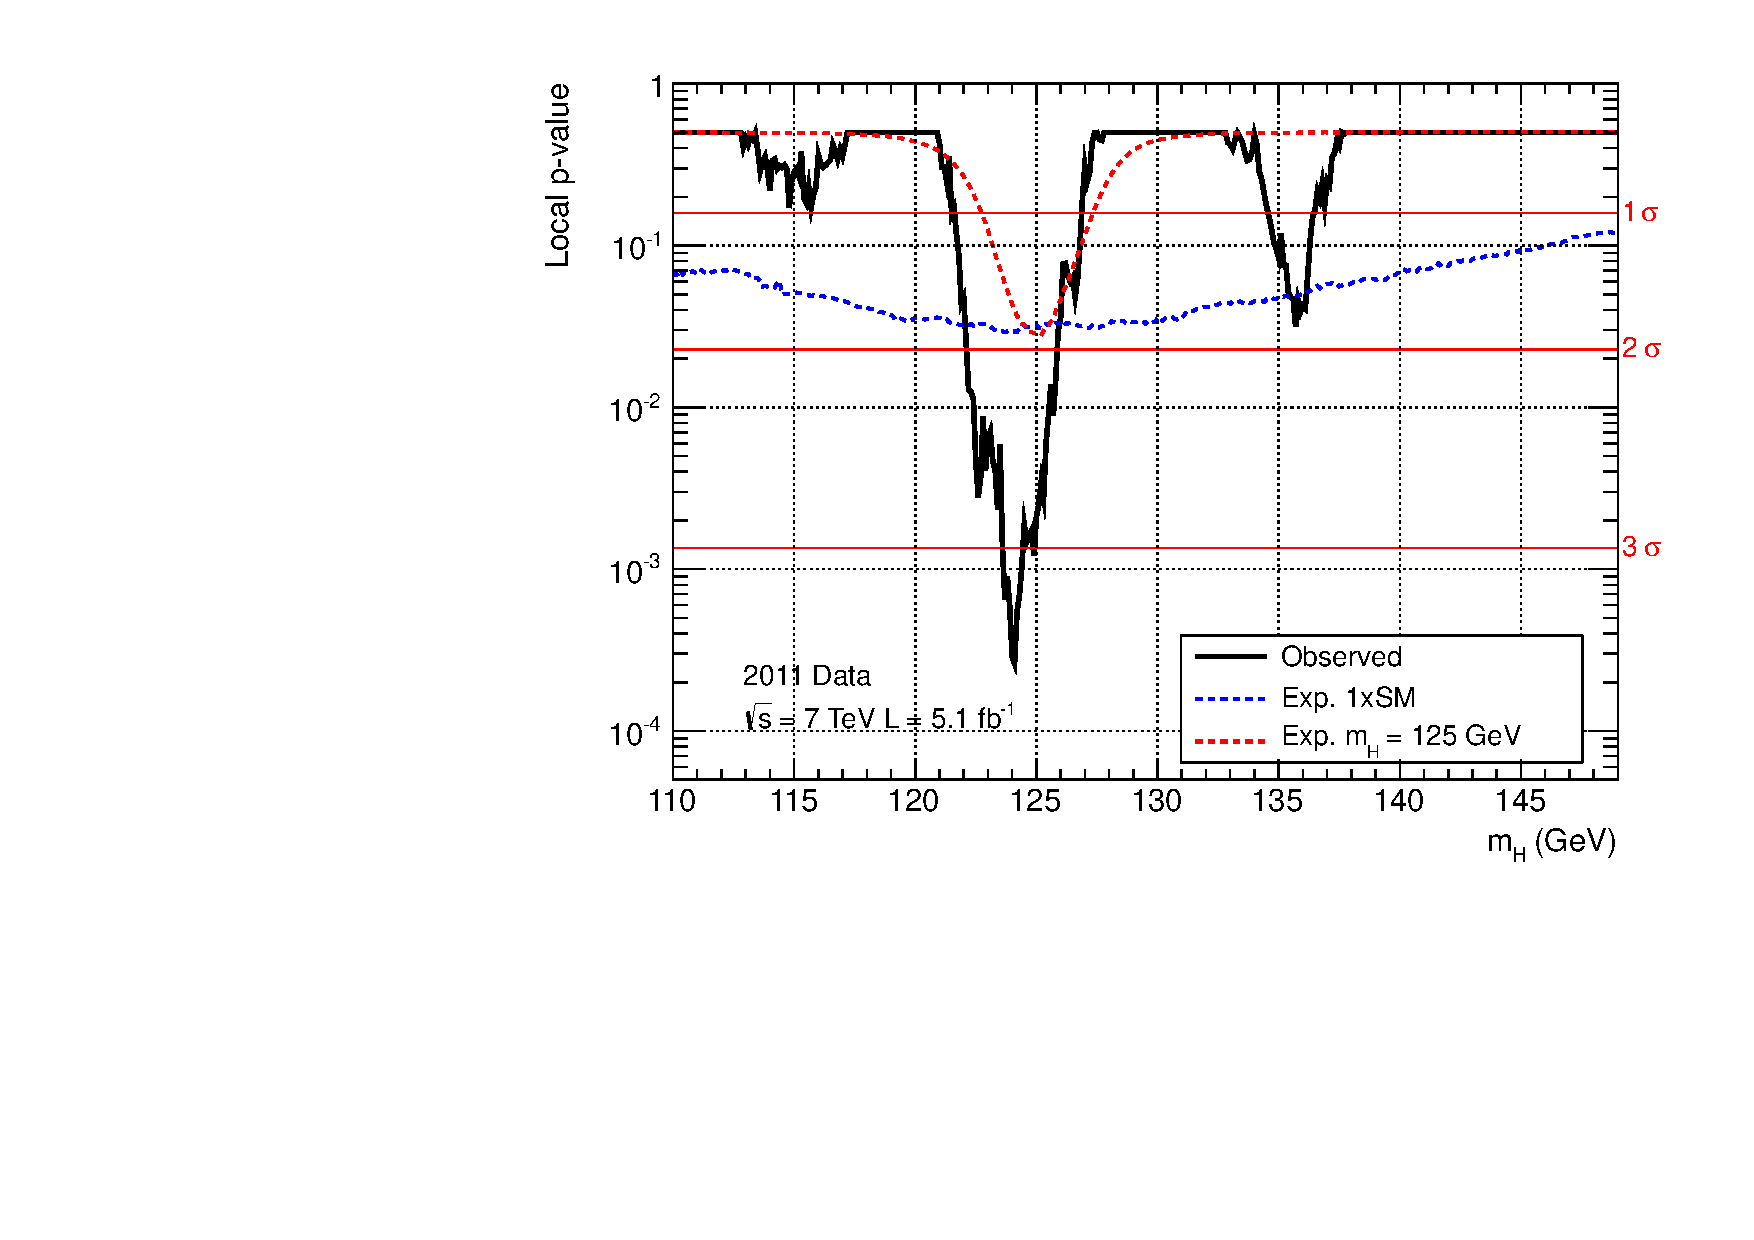
\includegraphics[width=.8\textwidth]{hgg7TeV/statsPlots/pvals-100MeV.pdf}
\end{center}
 \caption{Local p-value ($p_{0}$) calculated in steps of 100 MeV in the range $110<\mh<150$. 
 The observed $p_{0}$ obtained from the data is shown in black while the expected value in the presence of a
 SM Higgs boson is given by the dashed blue line. The expectation from a Higgs boson with mass 125 GeV is shown as a red
 dashed line. The right hand scale shows the significance in standard deviations at each $\mh$.}
 \label{fig:pvals7TeV}
\end{figure}

\begin{figure}
\begin{center}
  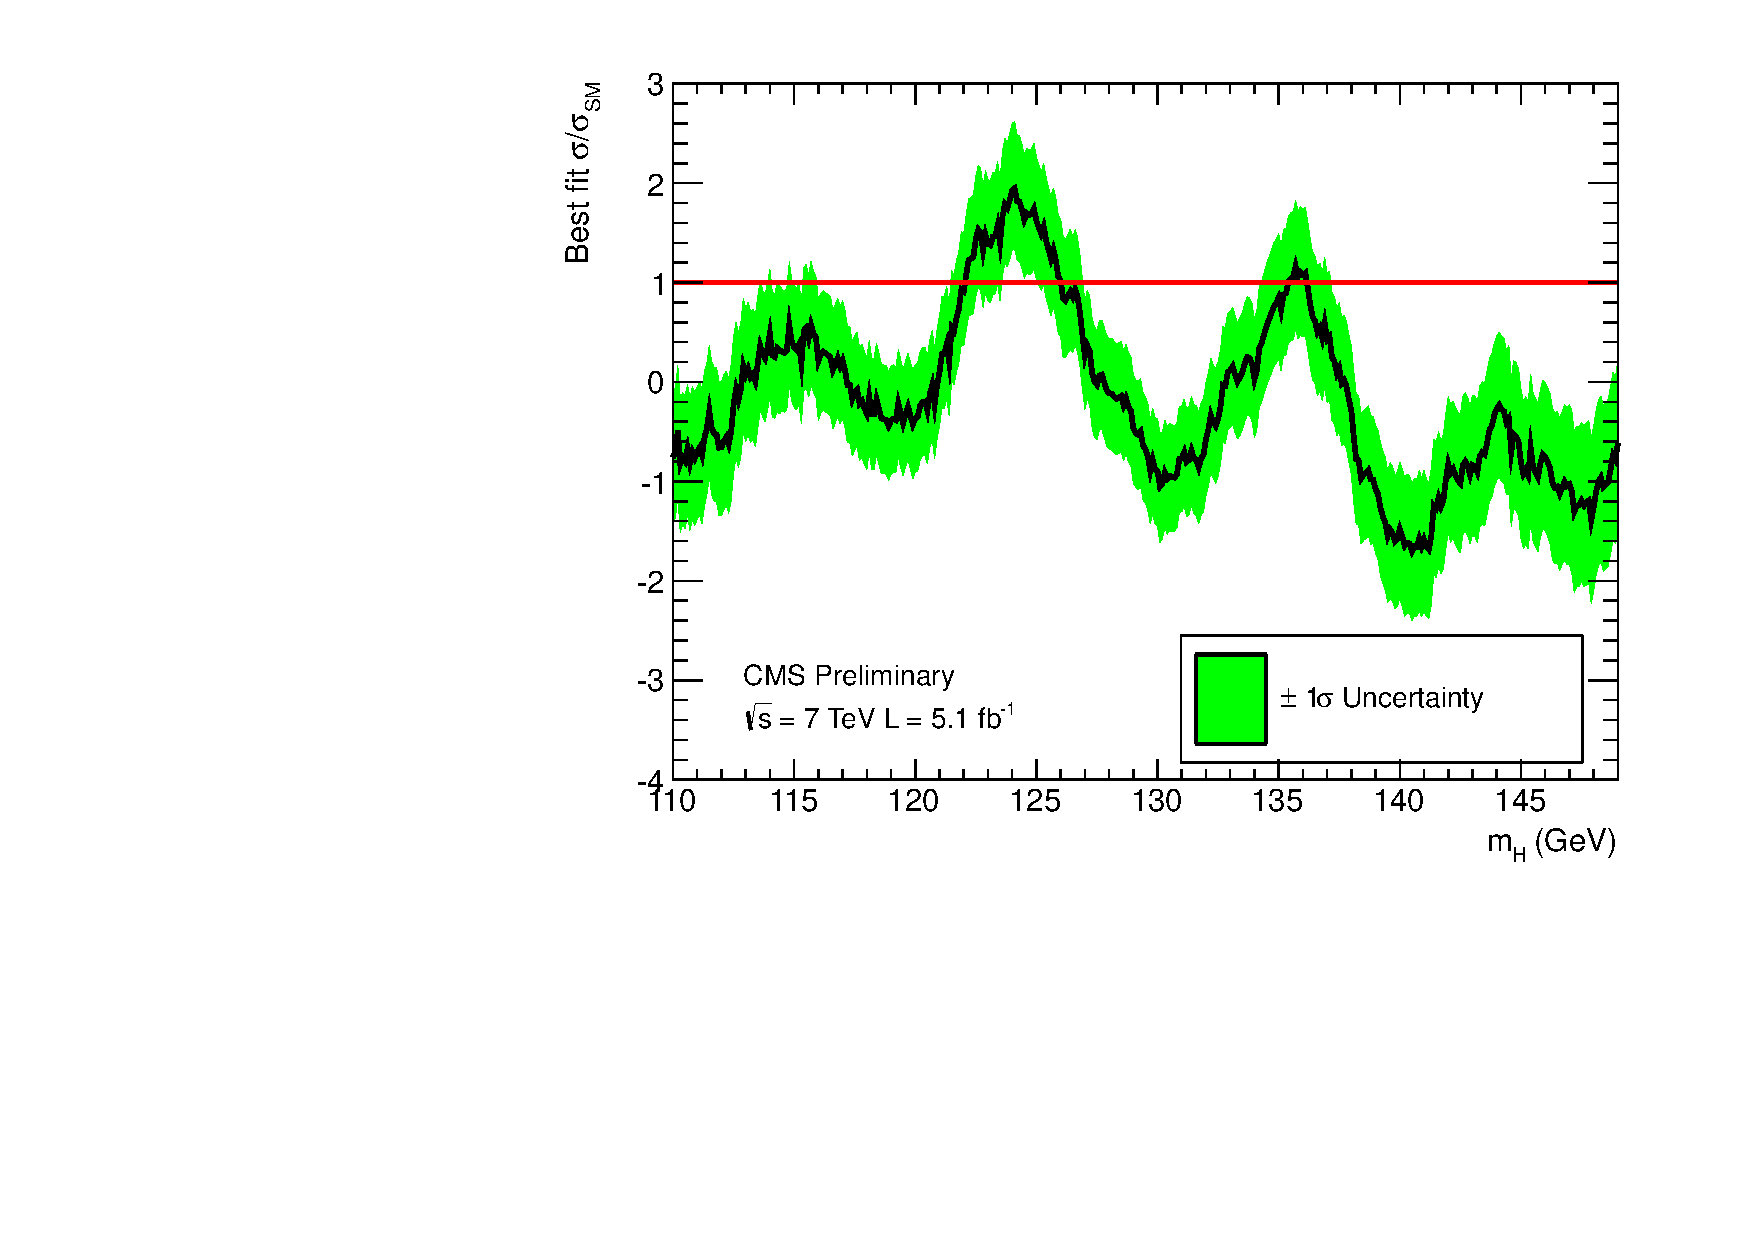
\includegraphics[width=.8\textwidth]{hgg7TeV/statsPlots/maxlh-100MeV.pdf}
\end{center}
 \caption{Best fit for the signal strength, $\muhat$, in steps of 100 MeV in the range $110<\mh<150$.
 The green bands indicate the 68\% uncertainty on $\muhat$ for a fixed $\mh$.
 The red line at 1 represents the expectation for a SM Higgs boson.}
 \label{fig:muhat7TeV}
\end{figure}

\subsubsection{The Look-Elsewhere Effect}
 
As the signal for the decay $\Hgg$ is a narrow mass peak, the probability to observe a local excess
anywhere in the search range is much larger than the probability to find one at any particular $\mh$.
This is an example of the look-elsewhere effect~\citep{leelyon}.
Due to this, the local p-value must be modified so as to 
express the probability to find an excess at least as significant as the one seen in data for all values of
$\mh$. This is done by throwing background-only pseudo-experiments 
and finding the minimum $p_{0}$ across all values of $\mh$ searched over. The fraction of pseudo-experiments with a minimum
$p_{0}$ less than the one observed in data is then the global p-value. 
Figure~\ref{fig:leestudy} shows the relationship between local and global p-values. The red line shows a 
fit of the function,
\begin{equation}
p_{global} = p_{local} + Ce^{ \frac { -Z^{2}} {{2} } },
\label{eqn:lee}
\end{equation}
where $Z$ is the local significance and $C$ is a free parameter~\citep{lee}. This function is then used to 
determine the look-elsewhere effect for larger significances.
The excess observed at 124 GeV corresponds to a global significance of $2.4\sigma$.

\begin{figure}
\begin{center}
  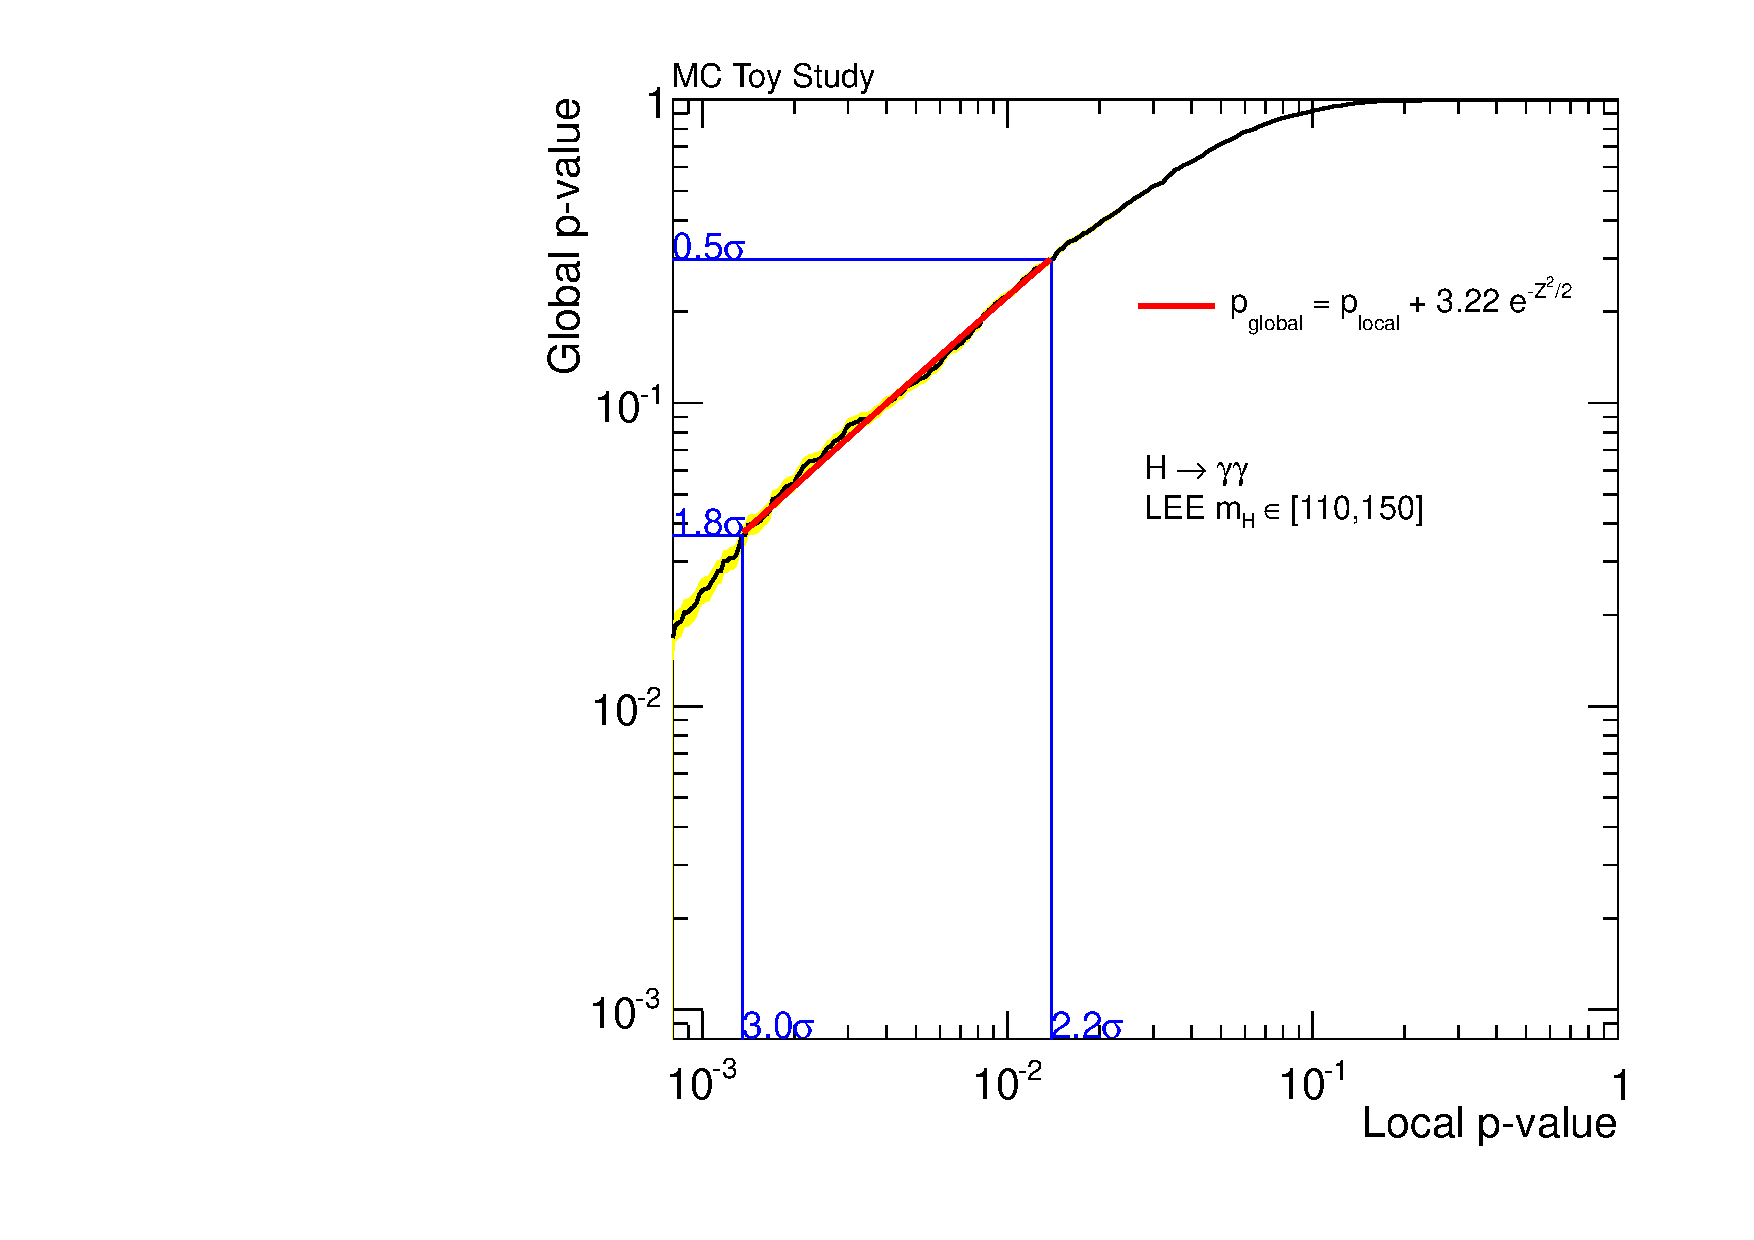
\includegraphics[width=.8\textwidth]{hgg7TeV/statsPlots/lee-extrap.pdf}
\end{center}
 \caption{Relationship between local and global p-values to determine the look-elsewhere effect 
 in the $\Hgg$ search for the range 110 to 150 GeV.
 The yellow band indicates the statistical precision of the relationship due to the limited number of toys
 produced. The red line indicates a fit of an analytic relation between the two and is used to calculate
 the global p-value for larger local significances.}
 \label{fig:leestudy}
\end{figure}

In order to generate suitable background-only toys, pseudo-data are generated in two variables, 
$\mgg$ and the diphoton BDT output. The value of $\mgg$ for each event in the pseudo-data 
is generated from a sum of two power laws which is 
fit to the full $\mgg$ spectrum in data in the range $100 < \mgg < 180$ GeV. The value of the diphoton BDT 
is generated by fitting a kernel density estimator to the distribution in data. The value of $\dmom$ is then 
calculated for each pseudo-event at every $\mh$ and the pseudo-dataset is analysed using the usual likelihood
of Equation~\ref{eqn:likelihoodhggbdt}. This approach is necessary to maintain
the correlations in the likelihood between neighbouring mass-hypotheses.


\subsection{Inclusion of 2012 Data}
\label{sec:8tev}

The search described in Chapter~\ref{chap:hgg} was repeated on data collected at CMS 
during the 2012 proton-proton run of the LHC, up to the time of the ICHEP conference in July 2012,  
at a center-of-mass energy of 8 TeV. The additional 
data were combined with the 7 TeV dataset as separate categories. 
The following section contains the results from the combined datasets corresponding to a 
total integrated luminosity of \clumicomb~\cite{HIG-12-028}.
% May want to expand on stuff here, only specifically on the changes to the analysis

\subsection{Updates for the 8 TeV Analysis}
\label{sec:updates8TeV}

The majority of the analysis remains unmodified between the two data taking periods.
Due to increased pileup conditions in the 2012 data, the regression BDTs and vertex BDTs
were re-trained using MC weighted to a higher average number of pileup vertices. 
As a result of this, both the diphoton and event categorisation BDTs were re-trained 
to incorporate the changes. In addition, the slight variation in kinematics between 
centre-of-mass energies of 7 and 8 TeV are accounted for in the retraining.
The isolation input variables to the photon ID BDT were modified, removing the correction
for the average energy density in the event, $\rho$. 
Instead $\rho$ was introduced as an additional input
variable so that the correlation between the number of pileup vertices and the isolation
could be taken into account in the BDT training. 

Both the energy scale and resolution were re-measured for the 2012 dataset and the corrections
applied to data and MC as with the 2011 analysis. The invariant mass cut on the dijet system for 
the dijet tagged events category was reduced to $250$ GeV, increasing the acceptance of $qqH$ production.
The dijet events were further subdivided by separating events with a large reconstructed dijet mass,
improving the sensitivity of the search. For the analysis described in Section~\ref{sec:signalextraction}, 
this results in two dijet bins with one being the tight class, containing dijet events with $m_{jj}>500$ 
GeV and the other loose class containing all other dijet events.
Figure~\ref{fig:results8TeV} shows the observed number of events from the 2012 dataset in each 
of the BDT output bins and the two dijet categories for $\mh=125$ GeV. The background model is derived 
using the procedure described in Section~\ref{sec:backgroundmodel} using the 2012 dataset. 
The contribution expected from a SM Higgs boson is shown in red. 

\begin{figure}
\begin{center}
  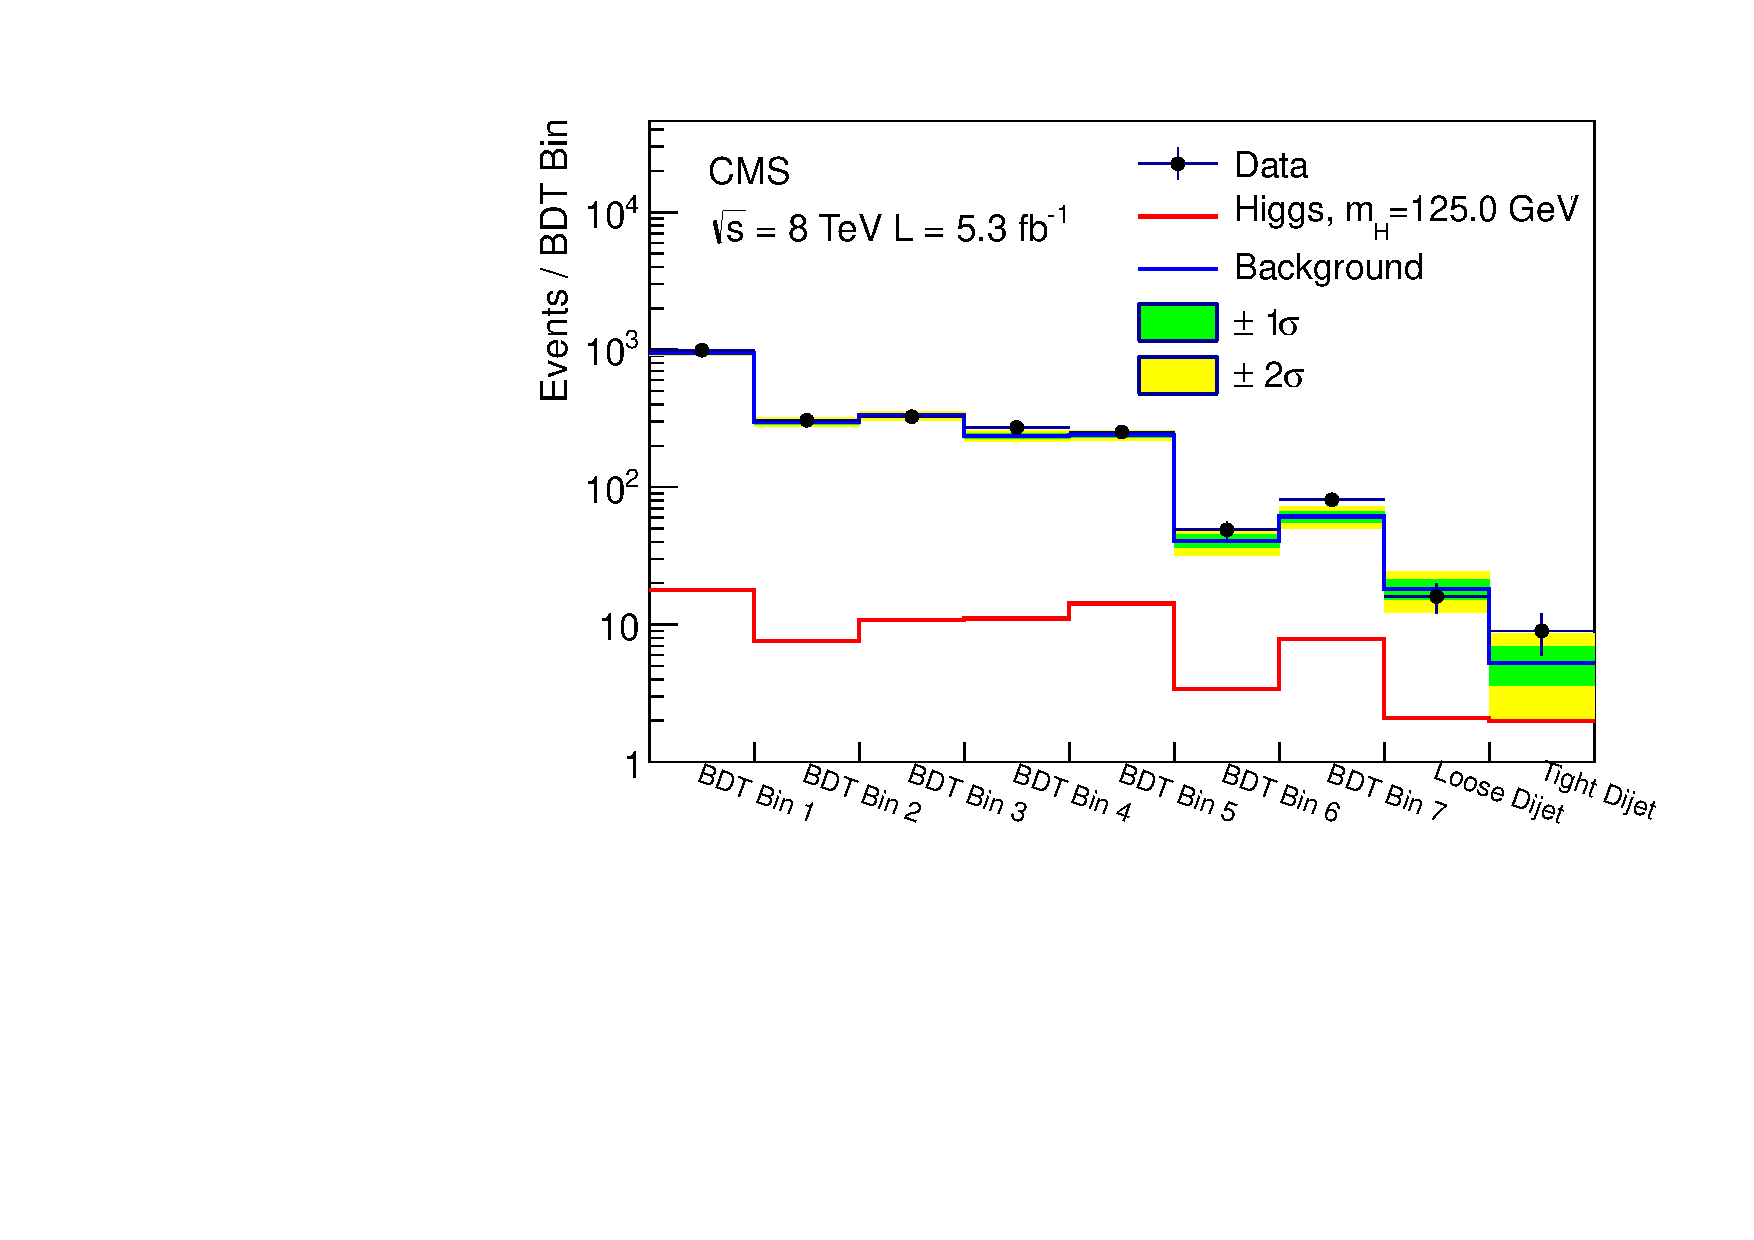
\includegraphics[width=.8\textwidth]{hgg8TeV/hgg_MassWindow_model_m125_8TeV.pdf}
\end{center}
 \caption{Observed number of events in the 2012 dataset for each of the seven BDT bins and tight/loose dijet bins
 for $\mh=125$ GeV. The background model is shown in blue along with the maximal $\pm 1/2\sigma$ variations.
 The expected contribution from a SM Higgs boson is shown in red~\citep{HIG-12-036}.}
 \label{fig:results8TeV}
\end{figure}

\subsection{Results from the Combined Datasets}
\label{sec:resultscombined}

The 2011 and 2012 datasets were combined statistically by extending the likelihood in 
Equation~\ref{eqn:likelihoodhggbdt}
to include a new set of categories which correspond to the updated analysis for the 2012 dataset.
By including the additional data as separate categories, 
exclusion limits and p-values are calculated as described in Section~\ref{sec:statisticalinterpretations}.
Figure~\ref{fig:limits8TeV} (left) shows the expected and observed 95\% upper limits 
on $\xsbr$ calculated in half GeV steps in $\mh$
from the combined datasets. The observed local p-value, $p_{0}$, determined
for the 7 TeV, 8 TeV and combined datasets, as a function of $\mh$ is shown in Figure~\ref{fig:limits8TeV} (right).
The largest excess is observed at $\mh=124$ GeV, corresponding to a local significance of $4.8\sigma$.
This is reduced to a global significance of $3.9\sigma$ when considering the look-elsewhere effect in 
the range 110 to 150 GeV.

\begin{figure}
\begin{center}
  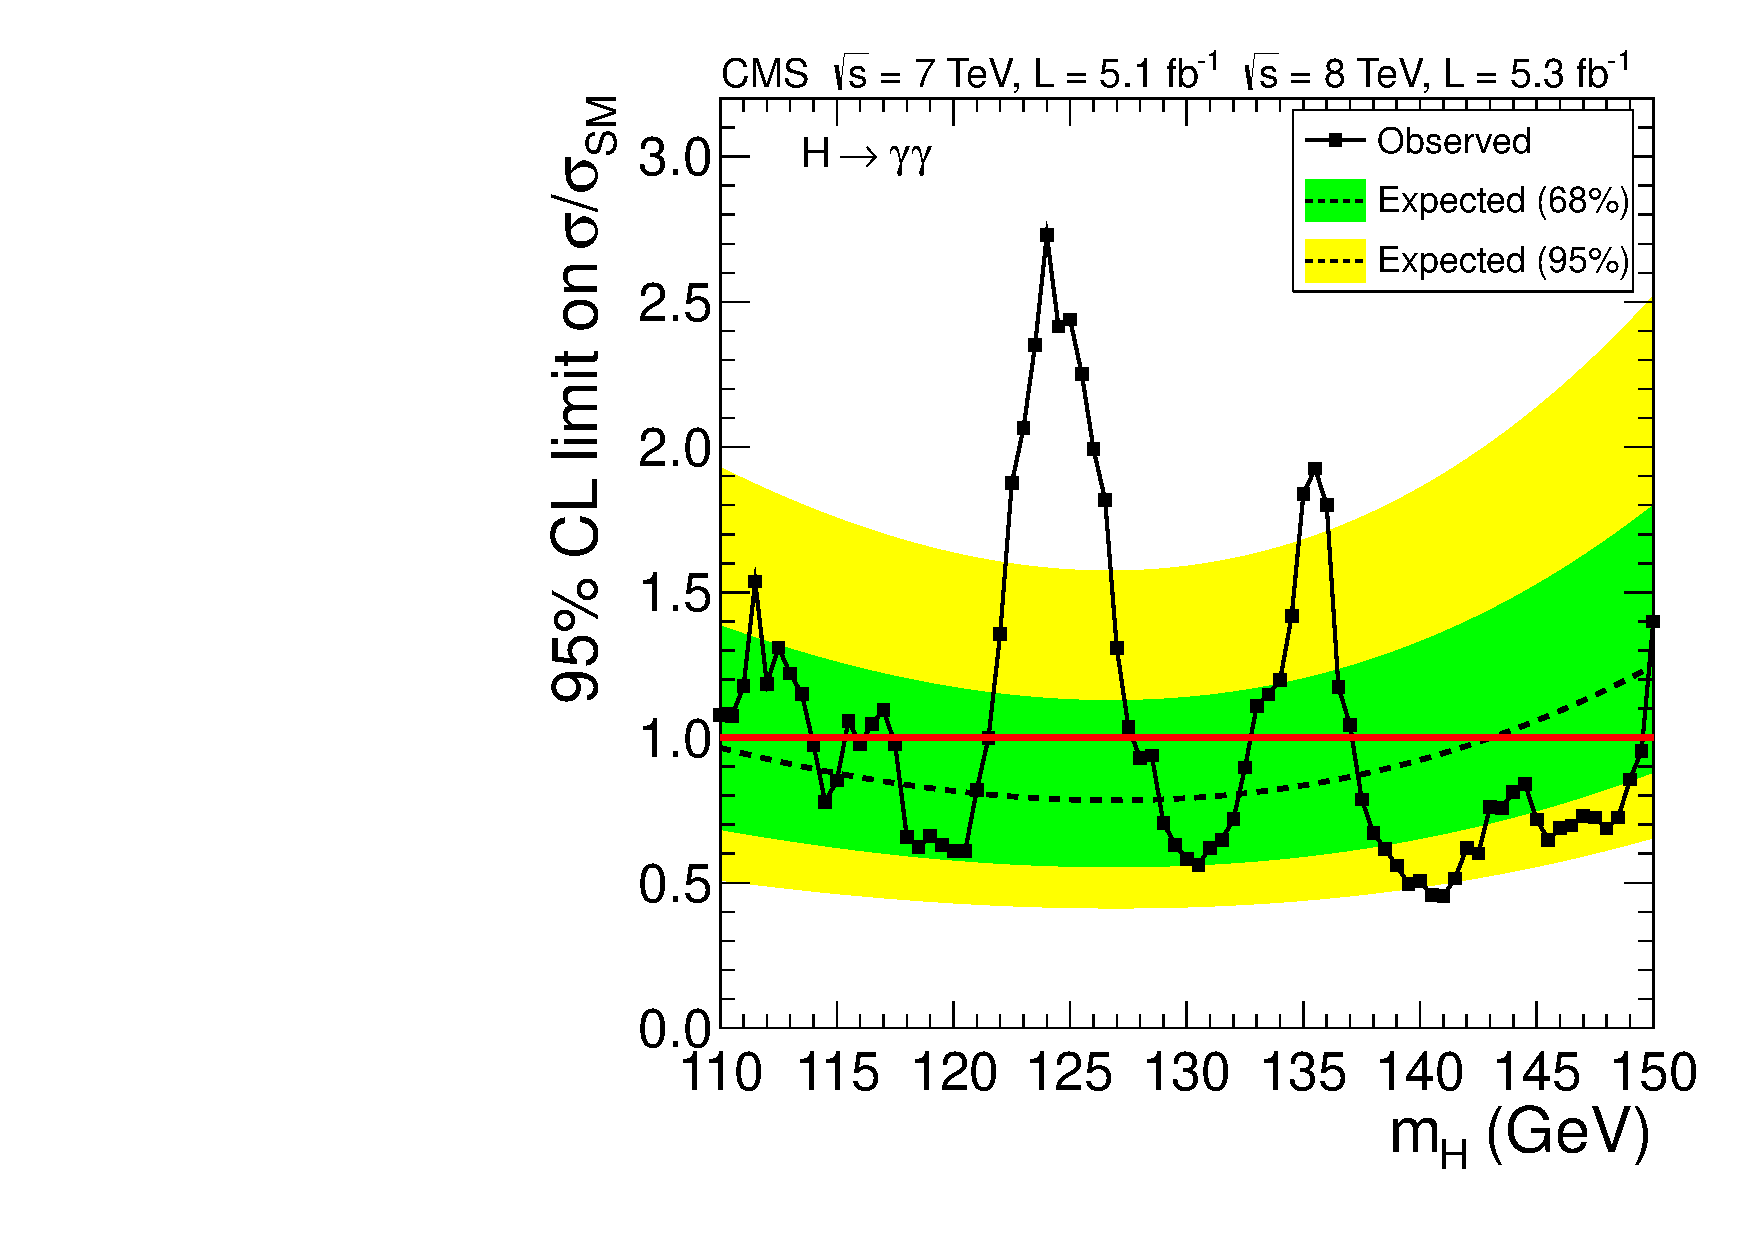
\includegraphics[width=.49\textwidth]{hgg8TeV/hgg_MassWindowLimit.pdf}
  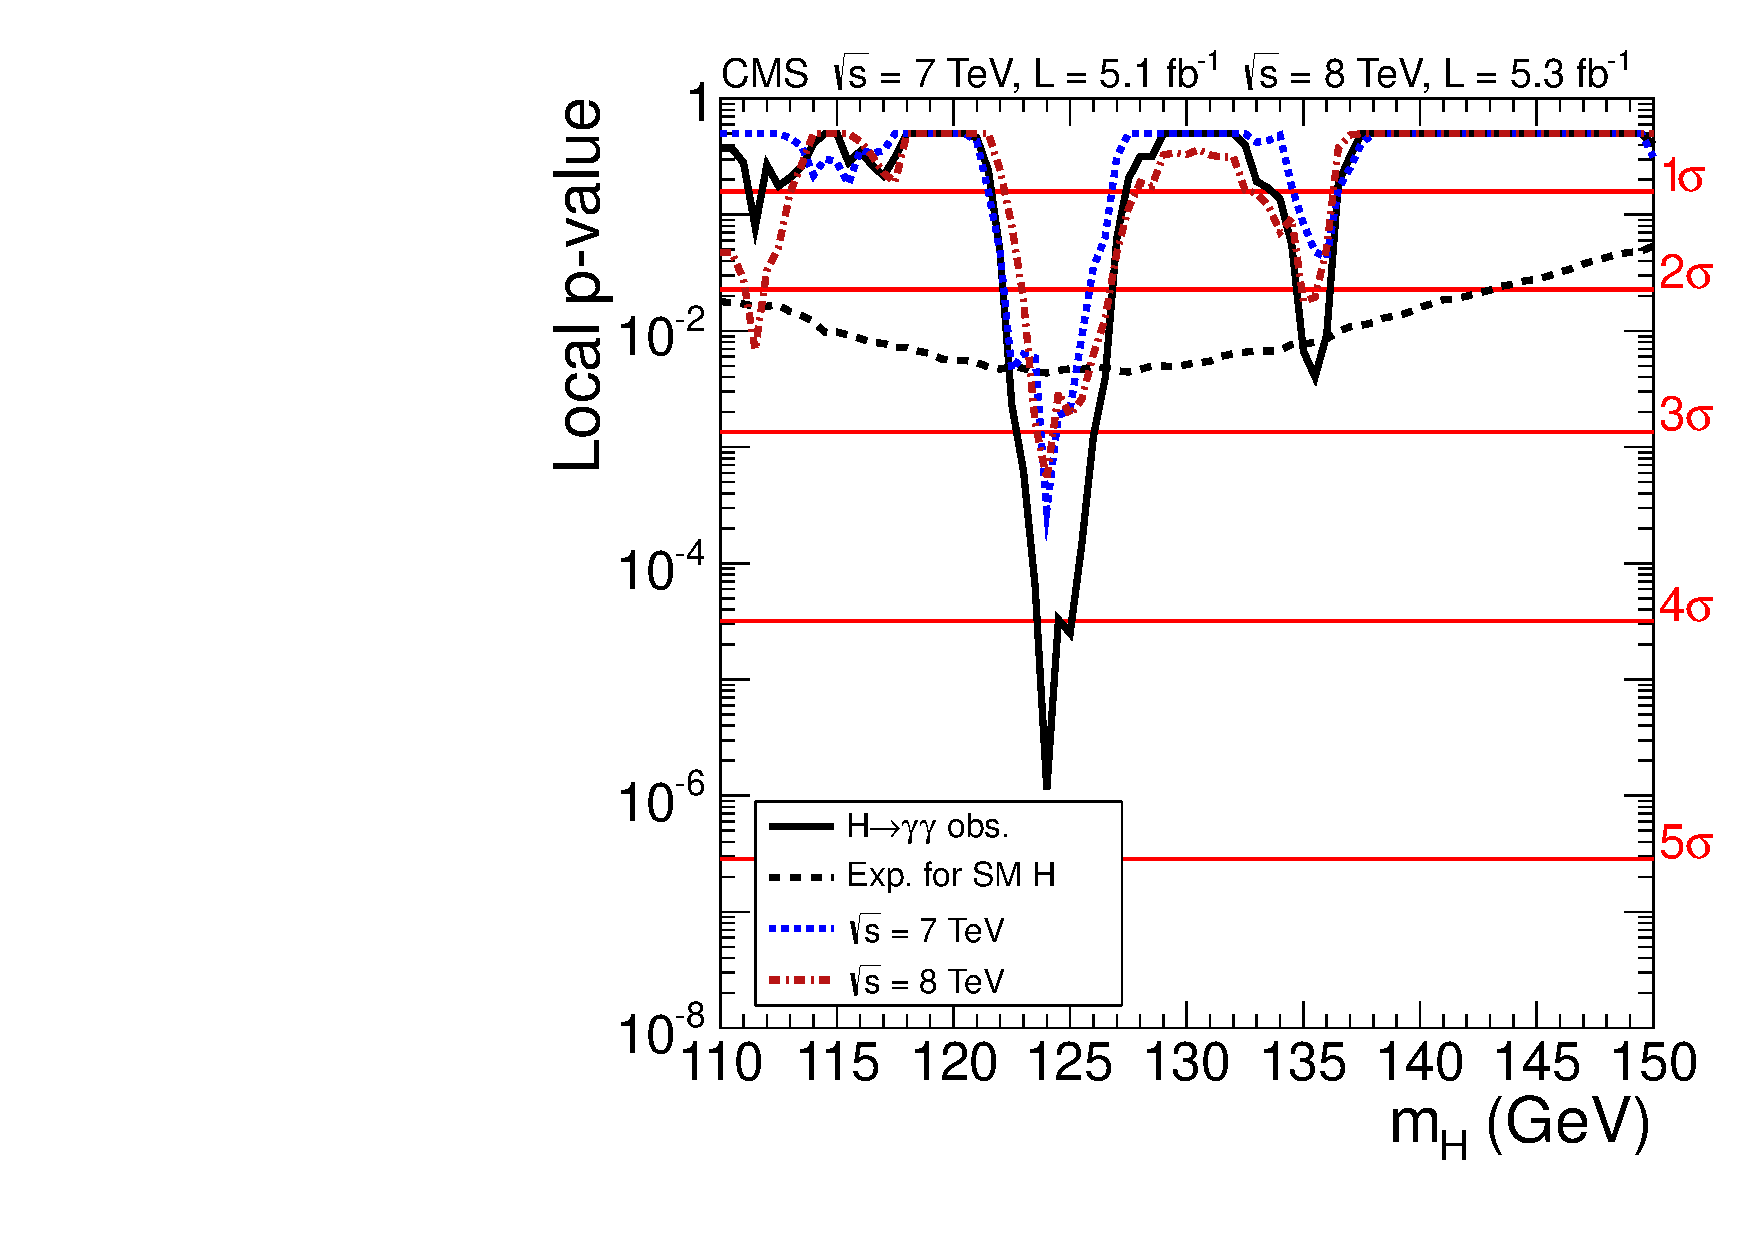
\includegraphics[width=.49\textwidth]{hgg8TeV/hgg_MassWindowPValue.pdf}
\end{center}
 \caption{Exclusion limits on SM Higgs boson production and subsequent decay to two photons
(left) and local p-value, $p_{0}$ (right) in the range
 $110 < \mh < 150$ GeV from the combined 2011 (7 TeV) and 2012 (8 TeV) datasets. 
 In the left figure, the black dashed lines indicates 
 the median expected value for the upper limit on $\mu$ 
 given the size of the dataset while the green and yellow bands indicate 
 the 68\% and 95\% quantile ranges respectively.
 The black solid line shows the observed upper limit.
 In the right figure, the observed $p_{0}$ obtained from the combined 
 datasets is shown in black while the expected value in the presence of a
 SM Higgs boson is given by the black dashed line. The observed $p_{0}$ from the 2011 (7 TeV) 
 and 2012 (8 TeV) datasets individually are shown by the 
 blue and red dashed lines respectively. The right hand scale shows the significance in 
 standard deviations at each $\mh$~\citep{HIG-12-036}.}
 \label{fig:limits8TeV}
\end{figure}


%\begin{figure}
%\begin{center}
% \caption{.}
% \label{fig:pvals8TeV}
%\end{center}
%\end{figure}
